\chapter{Social Media Data Acquisition}
In this section we describe the filtering process of the tweets and the creation of two lexicons. The food lexicon contains keywords with food related terms (e.g. \emph {rice, wheat, milk}) where the predictor lexicon contains keywords with factors influencing the price and supply of the goods (e.g. \emph{pricey}, \emph {cheap}, \emph{available}). We downloaded 2 TB of tweets from the internet archive \footnote{https://archive.org/details/archiveteam-json-twitterstream} over a span of October 2011 - September 2014.  The filtering process resulted with 5.6 M food relevant tweets.

Firstly, we detail an algorithm Hyperspace Analogue to Language (HAL)  \cite{lund96} which was used to find relevant keywords for our two lexicons. We then describe our framework for retrieving food related keywords that form our food lexicon followed by a chapter describing the framework for creating the Predictor Lexicon. In the Chapter Experimental Evaluation we analyse the different metrics influencing the performance of HAL and present the results. Lastly, we describe the filtering algorithm used to create our set of food relevant tweets.


\section{Hyperspace Analogue to Language}

HAL creates a semantic space from word co-occurrences \cite{lund96}. By using a sliding window parsing mechanism, the frequency of each term co-occurring within a fixed window size is recorded.  It is important to note that HAL only records the terms before the word we wish to analyse the context from. The terms after the word will appear in the column in the matrix that corresponds to that word.  The matrix is created by storing a vector for each word with the number of co-occurrences of every other word in the corpus. Hence, if our corpus contains $N$ different words the resulting HAL space would be an $N \times N$ square matrix of co-occurrences. Every time a specific word appears within the fixed window size the co-occurrence vectors are updated. For each co-occurrence HAL applies a scoring function. Words that appear closer, receive an inversely proportional score to its distance.

 To illustrate the idea \cite{burgess98} gives an example of a simple sentence \emph {"The horse raced past the barn fell."} in Table \ref{tab:halex} with a sliding window of five. Let's consider the first row.  \emph{"The"} precedes \emph{"Barn"} twice. Once within a distance of five and the other time it directly precedes the word  \emph{"Barn"}. Hence, that cell receives a score of five for the proximate one and a score of one for the word further away resulting in a final score of six. 

Following the creation of the matrix we concatenate both the column and row vector of a word, where the former represents the preceding words and the later the following. To compare the distance of the vectors we used the cosine similarity function. 

 



\begin{table}[h]
\centering
\begin{tabular}{ c c c c c c} \toprule
  & Barn & Horse &  Past & Raced & The \\ 
  \hline
 Barn &  & 2 &  4 & 3 & 6 \\ 
 Fell & 5 & 1 &  3 & 2 & 4 \\ 
 Horse &  &  &   &  & 5 \\ 
 Past &  & 4 &   & 5 & 3 \\ 
 Raced &  & 5 &   &  & 4 \\ 
 The &  & 3 &  5 & 4 & 2 \\ 
   \bottomrule
\end{tabular}
\caption{Toy example of HAL}
\label{tab:halex}
\end{table}


\subsection{Motivating a Semantic Approach}
\label{subsec:hal}

HAL gives us a way to study the relationship between words.  More specifically we aim to understand what words are represented in the context of \emph{Food} and topics centered around \emph{Food Security}. To achieve this we need a methodology for representing the meaning of a word. The reason that we analyse the context of a word is to identify new words that have a similar meaning or given the same context express the same thing. The later is concerned with identifying synonyms where as the former looks at contextual similarity. For example, let's look at the word \emph {mold} and \emph {available}. Those two words seem unrelate, but given the context of food they express the same thing.  Namely an abundance of food. Through the role  of the context they posses elements of items similarity but by themselves they would never be considered words with similar meaning. It's important to stress that they are not similar because they occur frequently locally, but because they occur frequently in similar sentential context. Burgess et al. \cite{burgess98} argues that a simple local co-occurrence analysis misses to capture a lot of relationships. For example the word street and road are basically synonyms however the seldom locally co-occur. They do, however occur in the same context. This observation motivated us to deviate from the commonly used co-occurrence analysis an take a step further to improve the precision of our filtering framework. 




\section{Food Lexicon}

Initially we started with a simple list of food related keywords. To avoid ambiguities we will refer to the initial keyword list as $K_i$. As a first source for our set $K_i$ we used the most common traded food commodities as it would easily allow us to verify our results using the price dataset made available by IMF \footnote{http://www.imf.org/external/np/res/commod/index.aspx}. We further decided to include the ten most important staple foods that feed the world as defined by Allianz\footnote{http://knowledge.allianz.com/demography/health/?767/the-worlds-staple-foods}. 

We filtered the archive dataset using exact string matching on $K_i$. The distribution of the food related tweets showed that we need to categorise our lexicon in order to have sufficient data for further analysis. Where global keywords such as \emph{food} are highly represented, more specific keywords such as \emph{beef} occur infrequently. Other than the sparsity of the data we also have the problem of ambiguous keywords. \emph {Soy} is such a keyword that refers in English to the \emph{bean} and in Spanish to the verb \emph{to be}. To avoid such ambiguity we extended the term to make it distinct (e.g. \emph{Soy} $\to$  \emph{Soy Bean}). 

To create categories we chose to mimic the categorisation of the FAO  \footnote{http://www.fao.org/worldfoodsituation/foodpricesindex/en/}. FAO tries to measure the overall food fluctuation by five different food categories namely \emph{meat, dairy products, cereals, vegetable oil} and \emph {sugar}. The weighted average of those five categories as illustrated in \cite{fao13}  defines the international food price index. We additionally created a further category named \emph{Other Food of Interest}. This category contains general keywords (e.g. \emph{food, dinner or lunch}) and food keywords that cannot be assigned to one of the five categories, but frequently occur (e.g. \emph {coffee, tea}). To be considered frequently the set of tweets containing the keyword needs to be $> 1\%$ of the total sample. 

The six subsets  $s$ are $\in K_f$ where $s$ is one of the six categories mentioned above. $C$ is an imaginary set that contains the five categories \emph{meat, dairy products, cereals, vegetable oil, sugar}  each being a subset containing all possible food items belonging to a specific category (e.g. the subset dairy would contain all possible dairy products). If the following relationship holds  $k \in C$, where $k$ is a keyword, for any keyword $k \in K_i$, we consider $k \in K_f$. For all keyword $k \notin C$ the condition of it being frequent is evaluated and if true added to $K_f$.  Food commodities that could not be assigned to any of the six categories were discarded (e.g. \emph {orange, cocoa, onion}). Upon manual examination of the dataset we realised that people are much more likely to talk about a specific food product rather than the raw material. \emph{Cereals} are not a public interest. However products such as \emph{bread} or \emph {flower} occur much more frequently. The set $K_f$  was further enriched by using food products that have been identified by \cite{AbbarMW14} in set $K_f$ only $\forall$ $k   \in K_f$ that are also $\in C$ . To further improve our coverage of the six food categories we filtered for synonyms and contextual similar words using HAL. 

\subsection{Candidate Food Term Selection}

We took several  steps in order to improve our detection of the desired food commodities. $K_f$ was created as follows: 
\begin{description}
  \item[1.)] We add all keywords $k \in K_i$ to  $K_f$ only if $k \in C $ or $k$ is frequent 
  \item[2.)] Further we add all keywords $ k \in K_f$ to $K_f$ only if $k \in C$
  \item[3.)] We create a HAL space using a random subsample of 10\% from our initial collection with all keywords that occur $> 100$. $\forall c \in C $ we pick the keyword $k\in K_f$ that most frequently occurs over the entire sample and retrieve the top 500 similar terms. We hand select those that are $\in C$.
\end{description}

% We took several  steps in order to improve our detection of the desired food commodities. The first step we took was a simple context analysis. The basic premise our approach relies on is that words with similar meaning repeatedly occur with similar words preceding and following it. We took a sample of 10 \% and counted the frequency of the 500 most occurring nouns and hand selected those unambiguously related to food. Looking at the distribution of the food related tweets \textbf{ \ref{fig:keywordDistribution}} we realised that we would have to categorise our lexicon in order to have sufficient data for further analysis.
 
The keyword set $K_f$ was used to perform exact term matching on the tweets collected from the internet archive. The resulting set of keywords in $K_f$ forms our Food Lexicon.  



 
\begin{table}[h]   
\centering
\scriptsize 
\begin{tabular}{p{1.3cm}|p{10.7cm} rlr}\toprule
\pbox{1.3cm}{Lexicon / \\ Subset $s$\\} & Keywords (i: from initial set, e: from $K_f$ , h: from HAL space )  \\
\hline
& & \\
\pbox{1.3cm}{$K_i$ \\Food } & \pbox{10.7cm}{  meal (i), meals (i) ,food (i), foods (i), wheat (i), rice v, maize (i), carley (i), soybean (i), soy (i), meat (i) , beef (i), cattle (i), chicken (i), poultry (i), lamb (i), swine (i), pork (i), fish (i), seafood (i), shrimp (i), salmon (i), sugar (i), bananas (i), oranges (i), coffee (i), cocoa (i), tea (i), milk (i), yams (i), cassava (i), potatoes (i), sorghum (i), plantain (i), nuts (i), onion (i), salt (i), egg (i), dairy (i), cereals (i)  }    \\
& & \\
 

\hline
\hline

& & \\
\pbox{1.3cm}{$K_f$ \\ Meat }  & \pbox{10.7cm}{ meat (i), lamb (i), pork (i), swine (i), chicken (i), poultry (i), beef (i),  sausage (e), rib (e), pastrami (e), kidney (e), liver (e), ham (e), bacon (e), chorizo (e), salami (e), sheep (e), boeuf (e), oxen (e), kine (e), steak (e), cow (e), brisket (e), veal (e), tenderloin (e), sirloin (e), poulet (e), volaille (e), hot dog (h), hamburgers (h),  meatballs (h), burgers (h), goat (h), cattle v, turkey (h), pig (h)}  \\
 & & \\
\hline

& & \\
\pbox{1.3cm}{$K_f$ \\Cereals }  & \pbox{10.7cm}{ wheat (i), atta (i), starch (i), farina (i), bran (i), ethanol (i), biofuel (i), rice (i), corn (i), maize (i), ravioli (e),  barley (e), scotch (e), whisky (h), oat (h), bread (h), flour (h), gluten (h), pasta (h), noodles (h), beer (h)  }  \\
& & \\

\hline

& & \\
\pbox{1.3cm}{$K_f$  \\Oil }  & \pbox{10.7cm}{ coconut oil (i), corn oil (i), olive oil (i), palm oil (i),peanut oil (i), sunflower oil (i), rapeseed oil (i), 
                                                              safflower oil (i),soybean oi (i), sunflower oil (i), soybeans (i), soya (i), soy sauce (i), soja (i)  }  \\
& & \\

\hline

& & \\
\pbox{1.3cm}{$K_f$ \\ Sugar }  & \pbox{10.7cm}{ sugar (i),  sugarcane (i), syrup (e), energy drink (e), cola (e), chocolate (e), nestle (e), cookies (h), cupcakes (h) }  \\
& & \\
 \hline                                                      

& & \\
\pbox{1.3cm}{$K_f$  \\ Dairy }  & \pbox{10.7cm}{ dairy (i), egg (i), milk (i), kefir (e) , butter (e), yogurt (e), quark (e), mozzarella (e), cheddar (e), parmesan (e),  
 		             buttermilk (e), ricotta (e), feta (e), romano (e), provolone (e), colby (e), edam (e), eggnog (e), pimento (e), 
		             cheshire (e), roquefort (e), icecream (h), milkshake (h), cheese (h), cream (h)} \\
& & \\
           
\hline

& & \\
\pbox{1.3cm}{$K_f$ \\ Other}  & \pbox{10.7cm}{ meal (i), meals (i), food (i), foods (i), fish (i) , prawn (i), seafood (i), salmon (i), tea (i), coffee (i),  dinner (h), lunch (h), breakfast (h), dish (h), cuisine (h)}  \\
& & \\

 \bottomrule

\end{tabular}
\caption{ A Summary of the Evolution of our Food Lexicon}
\label{tab:abc}
\end{table}
 



\section{Predictor Lexicon}

From our basic food lexicon we proceeded to extract features that we can use to explain events around Food Security. The FAO measures food security based on four dimensions namely \emph{Access, Availability, Stability} and \emph{Utilisation}. Where \emph{Access} mostly captures the supply of food, \emph{Availability} is concerned with the affordability of the basic goods. \emph{Utilisation} captures the nutritional value of the food and lastly \emph{Stability} is a measure of the other three dimensions over time. For food security objectives to be realised, all four dimensions must be fulfilled simultaneously \cite{fao2008}. 


To model food security we focus our work on those four dimension namely \emph{Access, Availability, Utilisation} and \emph{Stability}. Together those predictor categories build the set $C_p$. Attempts have been made to capture Availability by the UN \cite{ungp2013}. 

We define the predictor category \emph{Access} by looking for tweets containing price as a keyword as in \cite{ungp2013} but improve the recall by including synonyms of \emph{price} that appear in the same context. \emph{Availability} was defined in similar fashion by matching keywords that appear in the context of food availability as in \cite{hum14}, however a different set of keywords was selected as described in the following chapters. Unlike \cite{AbbarMW14} we don't measure food Utilisation by observing the exact diet but capture the people's food needs. Lastly as a measure of \emph{Stability} we focused our attention on economic stability. Keywords in the context of  poverty were selected to match this predictor category similar to \cite{RePEc} \cite{hum14}.



\subsection{Candidate Predictor Term Selection}

Since HAL has not been extensively used in previous work for term selection we drafted two different frameworks which we evaluated. As a reminder $K_f$ refers to the set of terms in our Food Lexicon. $F_c$ on the other hand refers to a corpus drafted from all food relevant tweets. Finally the manual selection of the keywords was done through crowd flower \footnote{http://www.crowdflower.com/}. 


\textbf{Framework 1}

\begin{description}
  \item[1.)] $\forall k \in K_f$ choose the keyword k with the highest occurrence form the entire sample. Let's call it $k_{max}$  
  \item[2.)] $\forall w \in F_c $ perform a similarity measure with $k_{max}$
  \item[3.)] Retrieve the 500 most similar words and hand select the words that occurs in the synonym lexicon thesaurus for supply, price, poverty and needs. 
    \item[4.)] For each of those hand-selected words  apply HAL 
  \item[5.)] For each predictor category retrieve the 500 most similar words and let crowd workers select the relevant terms. 
    \end{description}

The high-level intuition of this procedure is as follows. The first step will give us the most prominent food term. This is most likely going to be something general such as the keyword \emph{"Food"}. Step 2 and 3 will allow us to identify the most contextual similar keywords for each category. So the keyword is retrieved that is most likely used to describe supply in the context of food. In step 4 and 5 we aim to retrieve similar words that could describe supply but maybe appear more frequently in different contexts. In other words, we aim to find synonyms here.   


\textbf{Framework 2}


\begin{description}
   \item[1.)] $\forall w \in F_c $ perform a similarity measure with the keywords supply, price, needs and poverty
  \item[2.)]  Retrieve the 500 most similar words and let crowd workers select the relevant terms  
  \end{description}

Instead of finding a keyword that is a synonym of a predictor category as in Framework 1 we simply use our predefined category names as a base to retrieve contextually similar words. 

For the discovery of predictor terms we will proceed with Framework 2 for three reasons. Firstly Framework 1 did not retrieve us the desired keywords for all categories. Secondly, between the results of Framework 1 and 2 there was a substantial overlap and lastly Framework 2 is more efficient to execute. This is particularly important since creating the HAL space is computationally very expensive. The final lexicon was further enriched by including synonyms from thesaurus \footnote{http://www.thesaurus.com/} for supply, need, poverty, and price. The terms of the final predictor lexicon are presented in Table \ref{tab:pred_lex} and for future reference we will refer to it as $K_p$




\subsection{Annotation and False Positive Removal of HAL Results}

The workers were presented with four different tasks, one for each category. For every task we asked the workers to classify the term as A. Relevant, B. Likely, C. Unlikely and D. Not in English. Since Overlaps may occur, particularly for the category price and supply as well as poverty and need we asked the workers to classify them as likely in order to detect to which category the word has a stronger association. 

The crowd task presented a number of challenges. In our first test run we counted a false positive rate of around 40 \%. This was due to the lack of quality control we imposed on the workers. We observed a large amount of random guesses and a poor level of english among some workers. Hence we selected workers from commonwealth countries and regions where the majority are native english speakers. We further created test questions which were manually selected to  avoid inattentive workers. Lastly we collected 3 independent annotations for every word and applied a majority to resolve disagreements. Due to the imposed additional costs through the multiple annotations per term we restricted our search for relevant keywords to the top 140 terms suggested by HAL.

\section{Experimental Evaluation}
\label{sec:exp_eval}

In order to increase the recall of HAL we evaluated the performance on three different sample sizes (10 \%, 20 \%, 40 \%) constituting a corpus of around 23M, 47M, 93M words respectively. Our corpus of food related tweets has a number of appealing properties as it covers a large vocabulary centered around food. Unlike most corpora that represent formal business reports or specialised dictionaries our food corpus represents everyday speech. This gives us a closer approximation on how people would talk in the context of our predictor categories. 

The initial set of words in our corpus was filtered only to contain those words that appear at least 100 times. Words occurring infrequent were discarded as well as stop words and punctuations. On a test sample of 10 \% we observed that around 10 \% of the tweets contain equal or less then 4 words which could impact the quality of the results. Hence, on the 40 \% sample we further excluded tweets that contain less or equal to 4 words. Using the words $w \in F_c$ we produced a N by N matrix with the co-occurrences for three different window sizes namely five, eight and ten to investigate if the window size has an impact on the result. According to \cite{lund96} a window size of 8 should yield the best results. However the nature of a tweet is very different from a classical text so it remains to see if this observation also holds for microbologs. Since vector similarity measures are sensitive to the magnitude of the vectors we normalised all the vectors to a constant length. Once the HAL space was created we applied the above described Framework 2 to retrieve the desired keywords for our four categories. 

\subsection{Results}

We manually assed the annotations produced by crowd flower to check for disagreements between the crowd workers an ourselves. For the category supply we rejected 26 from 69 (39\%), for price 4 (12.5\%) from 32, for needs 8 (7\%) from 113 and for poverty 14 (\%) from 106. \\
\\
The high disagreement for the supply category was due to the ambiguous design of our question in the crowd task. We asked workers to accept words that can be both indicative for supply and price (e.g. rise, high) which unfortunately was misunderstood as to include words that can be only indicative of price (e.g. expensive). \\
\\
Similar to \cite{olt15} we observe that crowdsource annotators applied a more narrow definition of of the predictor categories overlooking some keywords associated with the cateogries. For example the term market was missed as a price keyword. Tweets containing the word market could provide valuable information regarding the state of food security as it's commonly used to describe the price  mood of a commodity. \\
\\
Looking at Figure \ref{fig:price_supply} and Figure \ref{fig:poverty_needs} we can observe that for all categories HAL performed best for a window size of 10 which contradicts the findings of \cite{lund96}. Additionally we see that the smaller sample sizes consistently produce more relevant keywords then the large sample.  A larger sample sizes increases the likelihood of a keywords occurrence. Since we set a fixed threshold of 100 occurrence across all samples we are more likely to include words with a smaller confidence , which might explain the poor performance. 


\begin{figure}[H]
        \centering
        \begin{subfigure}[b]{0.5\textwidth}
                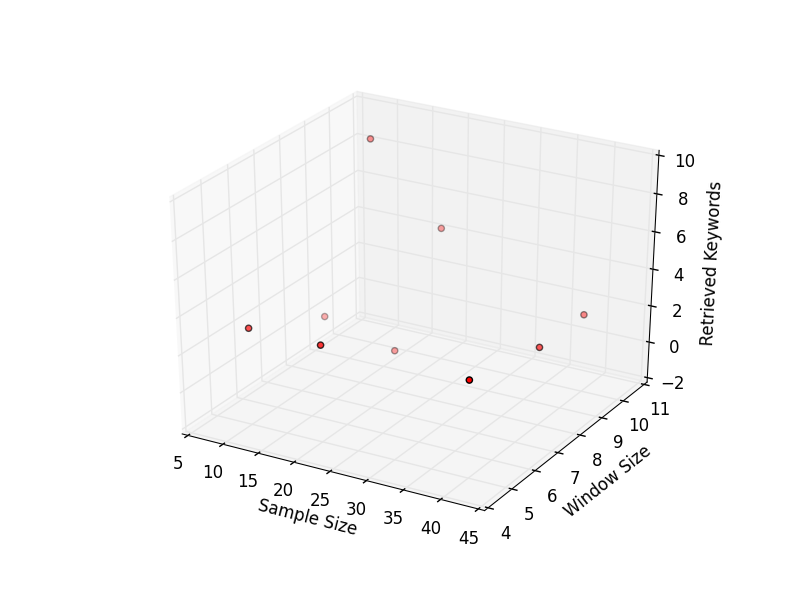
\includegraphics[width=\textwidth]{img/lex/price_hal}
                \caption{HAL - Price}
                \label{fig:al_price}
        \end{subfigure}%
        ~ %add desired spacing between images, e. g. ~, \quad, \qquad, \hfill etc.
          %(or a blank line to force the subfigure onto a new line)
        \begin{subfigure}[b]{0.5\textwidth}
                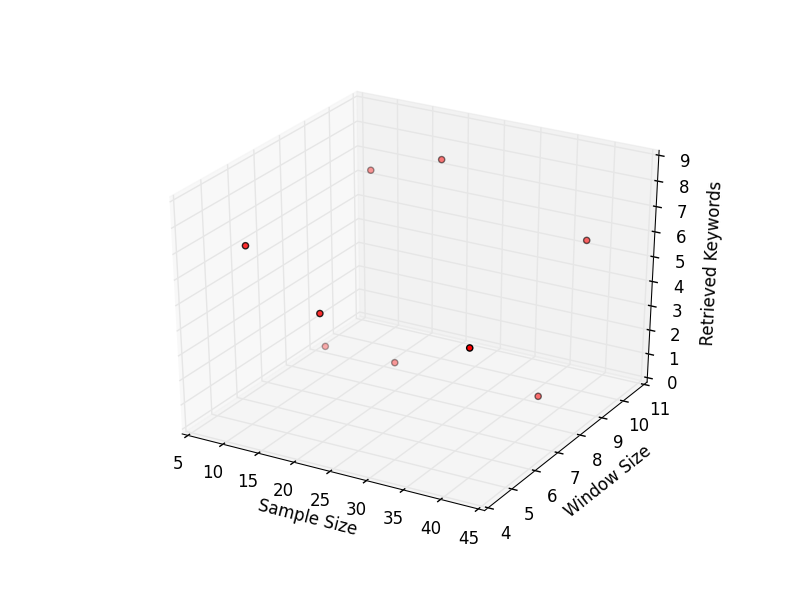
\includegraphics[width=\textwidth]{img/lex/supply_hal}
                \caption{HAL - Supply}
                \label{fig:hal_supply}
        \end{subfigure}
        ~ %add desired spacing between images, e. g. ~, \quad, \qquad, \hfill etc.
          %(or a blank line to force the subfigure onto a new line)
      
        \caption{HAL Evaluation for Price and Supply}\label{fig:price_supply}
\end{figure}


\begin{figure}[H]
        \centering
        \begin{subfigure}[b]{0.5\textwidth}
                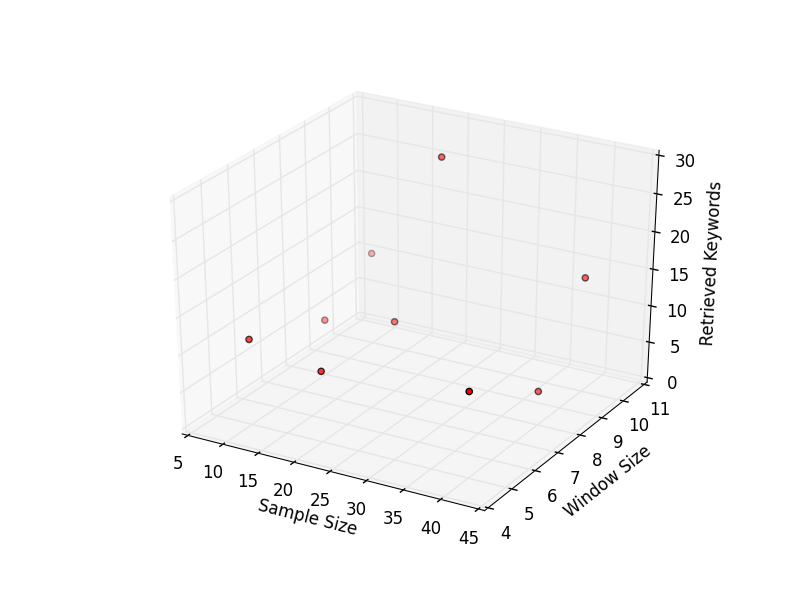
\includegraphics[width=\textwidth]{img/lex/needs_hal}
                \caption{HAL - Needs}
                \label{fig:al_price}
        \end{subfigure}%
        ~ %add desired spacing between images, e. g. ~, \quad, \qquad, \hfill etc.
          %(or a blank line to force the subfigure onto a new line)
       \begin{subfigure}[b]{0.5\textwidth}
                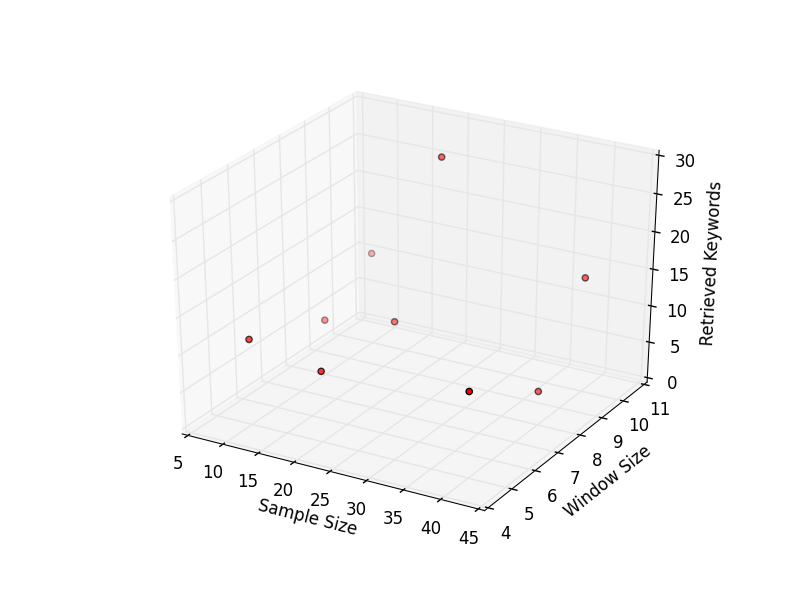
\includegraphics[width=\textwidth]{img/lex/needs_hal}
                \caption{HAL - Poverty}
                \label{fig:al_price}
        \end{subfigure}%
        ~ %add desired spacing between images, e. g. ~, \quad, \qquad, \hfill etc.
          %(or a blank line to force the subfigure onto a new line)
      
        \caption{HAL Evaluation for Poverty and Needs}\label{fig:poverty_needs}
\end{figure}

 
\subsection{Discussion}

We observed that HAL has a very high precision given a high similarity threshold. For the top 20 keywords we evaluated a precision of 100 \% for food relevant terms. In the top 20 we found other food items building the clear majority of the retrieved words. However the precision varies highly with the window and sample size. These variables, as our evaluation has shown, are very much dependent on the form of the corpus.  

With decreasing similarityt HAL highlighted some topics indirectly associated with food security. For example there was  a high percentage of country names in the retrieved results. Looking more closely at the retrieved countries we could see that most of them had a clear association to food. Where the majority of the retrieved countries such as Thailand, Bali \footnote{http://www.nomad4ever.com/2008/08/24/top-10-popular-foods-of-asia-explained/} or the cities Singapore and Paris \footnote{http://www.hellotravel.com/stories/best-food-cities-in-world} are considered to be famous holiday destinations for food lovers other retrieved countries such as Pakistan, Syria, Jakarta India or the Philippines \footnote{http://foodsecurityindex.eiu.com/Country} are cities with a clear history of food insecurity and political unrest. 
 
\begin{table}[h]   
\centering
\scriptsize 
\begin{tabular}{p{1.3cm}|p{10.7cm} rlr}\toprule
\pbox{1.3cm}{Lexicon / \\ Subset $s$\\} & Keywords ( h: from HAL space, t: from thesaurus )  \\
\hline

& & \\
\pbox{1.3cm}{$Food$ \\ Supply }  & \pbox{10.7cm}{  \emph{supply}, item (h), stock (h), vendors (h), demand (h), provided (h), feeds (h), delivery (h), supply (h), industry (h), production (h), waste (h), source (h), stash (h), numbers (h), list (h), growing (h), stores (h), distribution (h), delivered (h), policy (h), purchases (h), market (h), processing (h), chain (h), packaging (h), network(h), mart (h), stalls (h), sustainability (h), aplenty (t), bags (t), bulk (t), bundle (t), chunk (t), expanse (t), extent (t), flock (t), chunk (t), expanse (t), extent (t), flock (t), gob (t), heap (t), hunk (t), jillion v, load (t), lot (t), magnitude (t), mass (t), meassure (t), mess (t), mint (t), mucho (t), oodles (t), pack (t), pile (t), scads (t), score (t), slat (t), slew (t), ton (t), volume (t) }  \\
 & & \\
\hline
& & \\
\pbox{1.3cm}{$Food $ \\Price }  & \pbox{10.7cm}{
\emph{price}, affordable (h), cost (h), rise (h), savings (h), coupons (h), prices (h), label (h), purchase (h), economy (h), discount (h), budget (h), sales (h), benefit (h), target (h), bonus (h), size (h), money (h), better (h), best (h), free (h), buy (h), amount (t), bill (t), , demand (t), estimate (t), expenditure (t), expense (t), fare (t), fee (t), figure (t), output (t), pay (t), payment (t), premium (t), rate (t), return (t), tariff (t), valuation (t), worth (t), appraisal (t) } \\
& & \\
\hline
& & \\
\pbox{1.3cm}{$Food $ \\Poverty }  & \pbox{10.7cm}{\emph{poverty},  appetite (h), rich (h), shelter (h), homeless (h), shortage (h), control (h), provide (h), feed (h), needy (h), edible (h), nutrition (h), donate (h), 
expensive (h), economy (h), thought (h), budget (h), poor (h), service (h), supplies (h), crisis (h), demand (h), poverty (h), pantry (h), cravings (h),
 agricultural, resources, assistance, insecurity, storage (h), issue (h), bank (h), safety (h), prices (h), funding (h), health (h), drug (h), challenges (h), distribution (h), helping (h), government (h), affected (h), scraps (h), fair (h), children (h), support (h), waste (h), program (h), crops (h), restrictions (h), parcels (h), industry (h), healthcare (h), culture (h), catering (h), delicious (h), writer (h), sustainability (h), revolution (h),inflation (h), policy (h), daily (h), bankruptcy (t), debt (t), deficit (t), difficulty (t), famine (t), hardship (t), lack (t), scarcity (t), shortage (t), starvation (t),underdevelopment (t),
abundance (t), affluence (t), bounty (t), myriad (t),plenty (t), plethora (t), profusion (t), prosperity (t), riches (t), wealth (t)
  }  \\
& & \\
\hline
& & \\
\pbox{1.3cm}{$Food $ \\Needs }  & \pbox{10.7cm}{ 
\emph{need}, must (h), loving (h), share (h), like (h), favourite (h), hate (h), ordering (h), eat (h), give (h), much (h), want (h), needs (h), takes (h), beg (h), iwant (h), getting (h), favorite (h), buy (h), 50thingsilove (h), enough (h), ilove (h), whatilovethemost (h), got (h), horrible (h), cookout (h), poor (h), ate (h), deliver (h), neeeeed (h), looooove (h), neeed (h), neeeed (h), make (h), good (h), 2thingsilove (h), lack, tweetyourweakness, terrible, bring, ineed, lots (h), waiting (h), bit (h), starving (h), gave (h), delicious (h), drink (h), nice (h), cook (h), hungry (h), craving (h), healthy (h), wish (h), awesome (h), really (h), best (h), dearth (t), deficiency (t), drought (t), inadequacy (t), insufficiency (t), lack (t), need (t), omission (t), privation (t), unavailability (t), void (t), want (t),affluence (t), bounty (t), myriad (t), plenty (t), plethora (t), profusion (t), prosperity (t), riches (t), wealth (t), ampleness (t), copiousness (t), fortune (t), oppluence (t), plentitude (t), prosperousness (t)   }  \\
& & \\

\bottomrule

\end{tabular}
\caption{ Keywords of Predictor Categories}
\label{tab:pred_lex}
\end{table}
 
 \newpage
 

\section{Filtering}

The filtering of the tweets was performed in three rounds. First we filtered for food relevant tweets. In a second round we applied our Predictor Lexicon on the retrieved set of tweets obtained in the first step. Lastly we filter by sentiment. 

\subsection{Food related Tweets} 

The food related tweets were retrieved through exact term matching, i.e. a tweet containing the term \emph{foods} would not match on the keyword \emph {food} where the reverse is also true. We mimic the term matching twitter performs. In the initial round we optimised for coverage and hence avoided further filtering steps. Given the large size of the dataset efficiency was also a concern. We experimented with both string.split() and a tokenizer provided by the Natural Language Toolkit \cite{Loper2002}. String.split() proved to be more tweekable. The result was a collection of 5.6 M tweets posted by 4.2 M users. 

\subsection{Predictor related Tweets}

The first round  drastically reduced our dataset to around 90 GB of tweets. This allowed us to perform a more involved filtering mechanism similar to \cite{hum14}. 

For every word in a tweet and for every word in our predictor lexicon $K_p$ the stem was computed. This was necessary to capture tweets that may contain a predictor term that is not in its base form. Fore example a tweet containing the word \emph{pricey} would not match the term \emph{price}. Furthermore the framework also accounts for misspelt words. To do this in a computationally efficient way the algorithm computes the edit distance between a given word and terms from the predictor set D. If the error is within a fixed threshold the predictor term with the minimal edit distance is returned. 

\subsection{Sentiment Extraction}

Experiments in \cite{hum14} showed that sentiment analysers such as SentiStrength \cite{sent10} or Stanford CoreNLP \cite{stanford2011} performed  poorly on microblog content. Hence in \cite{hum14} the decision was made to extract the sentiment by having specific terms for each sentiment (polarity). In addition one had to account for changes in polarity through negations such as \emph{never} and \emph{not} which inverted the polarity of a predictor category term. 

We however choose to deviate from this approach and use a sentiment analyser despite the bad results. We give two reasons for doing so. 1.) Hutto et. al recently published a new sentiment analyser VADER \cite{hutton14} with an F1 Classification Accuracy = 0.96 which  outperformed human evaluators. 2.) Often keywords can not be manually assigned to a polarity without knowing it's context. 

Besides the above mentioned benefits VADER allows us to obtain a degree of sentiment by analysing grammatical and syntactical conventions that humans use when expressing sentiment intensity. For example it accounts for emoticons which are commonly used to express a sentiment or even acronyms such as \emph{LOL, WTF}. It's further worth mentioning that VADER is an unsupervised approach and is well suited for streaming data. 






\chapter{Analysis}






\section{Data Analysis}


\subsection {User Distribution}

Twitter is a social network and in general such networks follow a power law distribution \cite{Whittaker:1998}. We see in the bellow Figure \textbf{\ref{fig:u_linear}} and Figure \textbf{\ref{fig:u_log}}  that the distribution of the number of tweets per user slightly deviates from a normal power law. A lot of individuals  send only a few tweets about the subject and only a small number of users transmit a large amount of tweets. Unlike \cite{bild15} suggest the contribution participation level of  80 \%, 20 \%   does not seem to apply to tweets about food. In Figure \ref{fig:no_power} we can see that the curve is very flat. About 40 \% of the tweets are caused by 20 \% of the users. This deviates highly form the normally observed 80 \%, 20 \% ratio. We assume that this is due to the wide spread interest of the topic.

\begin{figure}[ht]
        \centering
        \begin{subfigure}[b]{0.5\textwidth}
                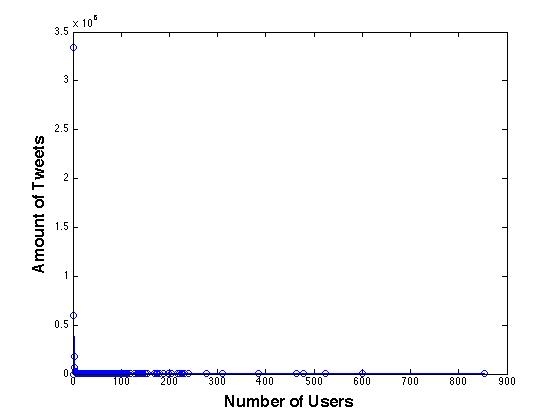
\includegraphics[width=\textwidth]{img/anal/linear_user}
                \caption{Linear: Number of Tweets per User}
                \label{fig:u_linear}
        \end{subfigure}%
        ~ %add desired spacing between images, e. g. ~, \quad, \qquad, \hfill etc.
          %(or a blank line to force the subfigure onto a new line)
        \begin{subfigure}[b]{0.5\textwidth}
                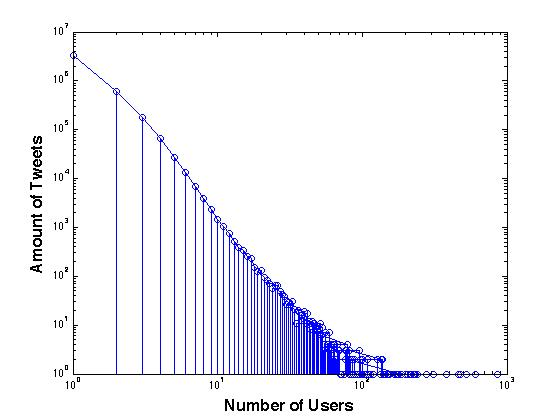
\includegraphics[width=\textwidth]{img/anal/loglog_users_tweets}
                \caption{LogLog: Number of Tweets per User}
                \label{fig:u_log}
        \end{subfigure}
        ~ %add desired spacing between images, e. g. ~, \quad, \qquad, \hfill etc.
          %(or a blank line to force the subfigure onto a new line)
      \begin{subfigure}[b]{0.5\textwidth}
                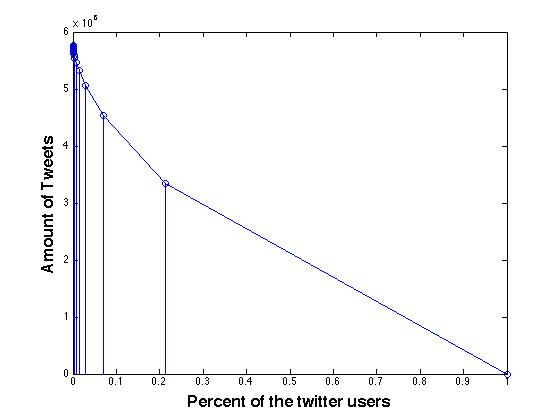
\includegraphics[width=\textwidth]{img/anal/no_power}
                \caption{Distribution: Number of Tweets per User}
                \label{fig:no_power}
        \end{subfigure}
        ~ %add desired spacing between images, e. g. ~, \quad, \qquad, \hfill etc.
          %(or a blank line to force the subfigure onto a new line)

      
        \caption{Volume of Tweets per Keyword and per Category}\label{fig:distribution}
\end{figure}

\subsection {Food Term Distribution}

Our framework for the data acquisition successfully increased the total volume of food related tweets. From an initial 2.6 M tweets we raised the entire volume by 110\% to a total of 5.6 M food related tweets. The distribution of the volume per food term is displayed in Figure \ref{fig:world}. We illustrate in orange the added volume alongside the initial size in blue. The most popular food terms on twitter are general terms such as food, dinner and lunch. Within the 10 most popular terms we found that three beverages (coffee, beer, tea) were represented. The most popular traded commodity term on social media is chicken.  We further show the distribution of the categories in \ref{fig:cat}. By far the highest contribution has the category \emph{others} due to general food related keywords such as \emph{dinner} or \emph{food}. It builds the absolute majority with 51 \%. Meat related keywords has the second highest contribution with around 15 \% followed by 12\% sugar, 11\%  cereals, 10 \% dairy  and lastly 0.2 \% Vegetable Oils. Interestingly the volume roughly follows the economic importance of the different categories with the only outlier being sugar \cite{fao2008}. We assume this is due to the highly popular products \emph{coca cola} and empty	{chocolate} which caused alone 70 \% of the sugar related tweets. 



\begin{figure}[H]
        \centering
        \begin{subfigure}[b]{0.5\textwidth}
                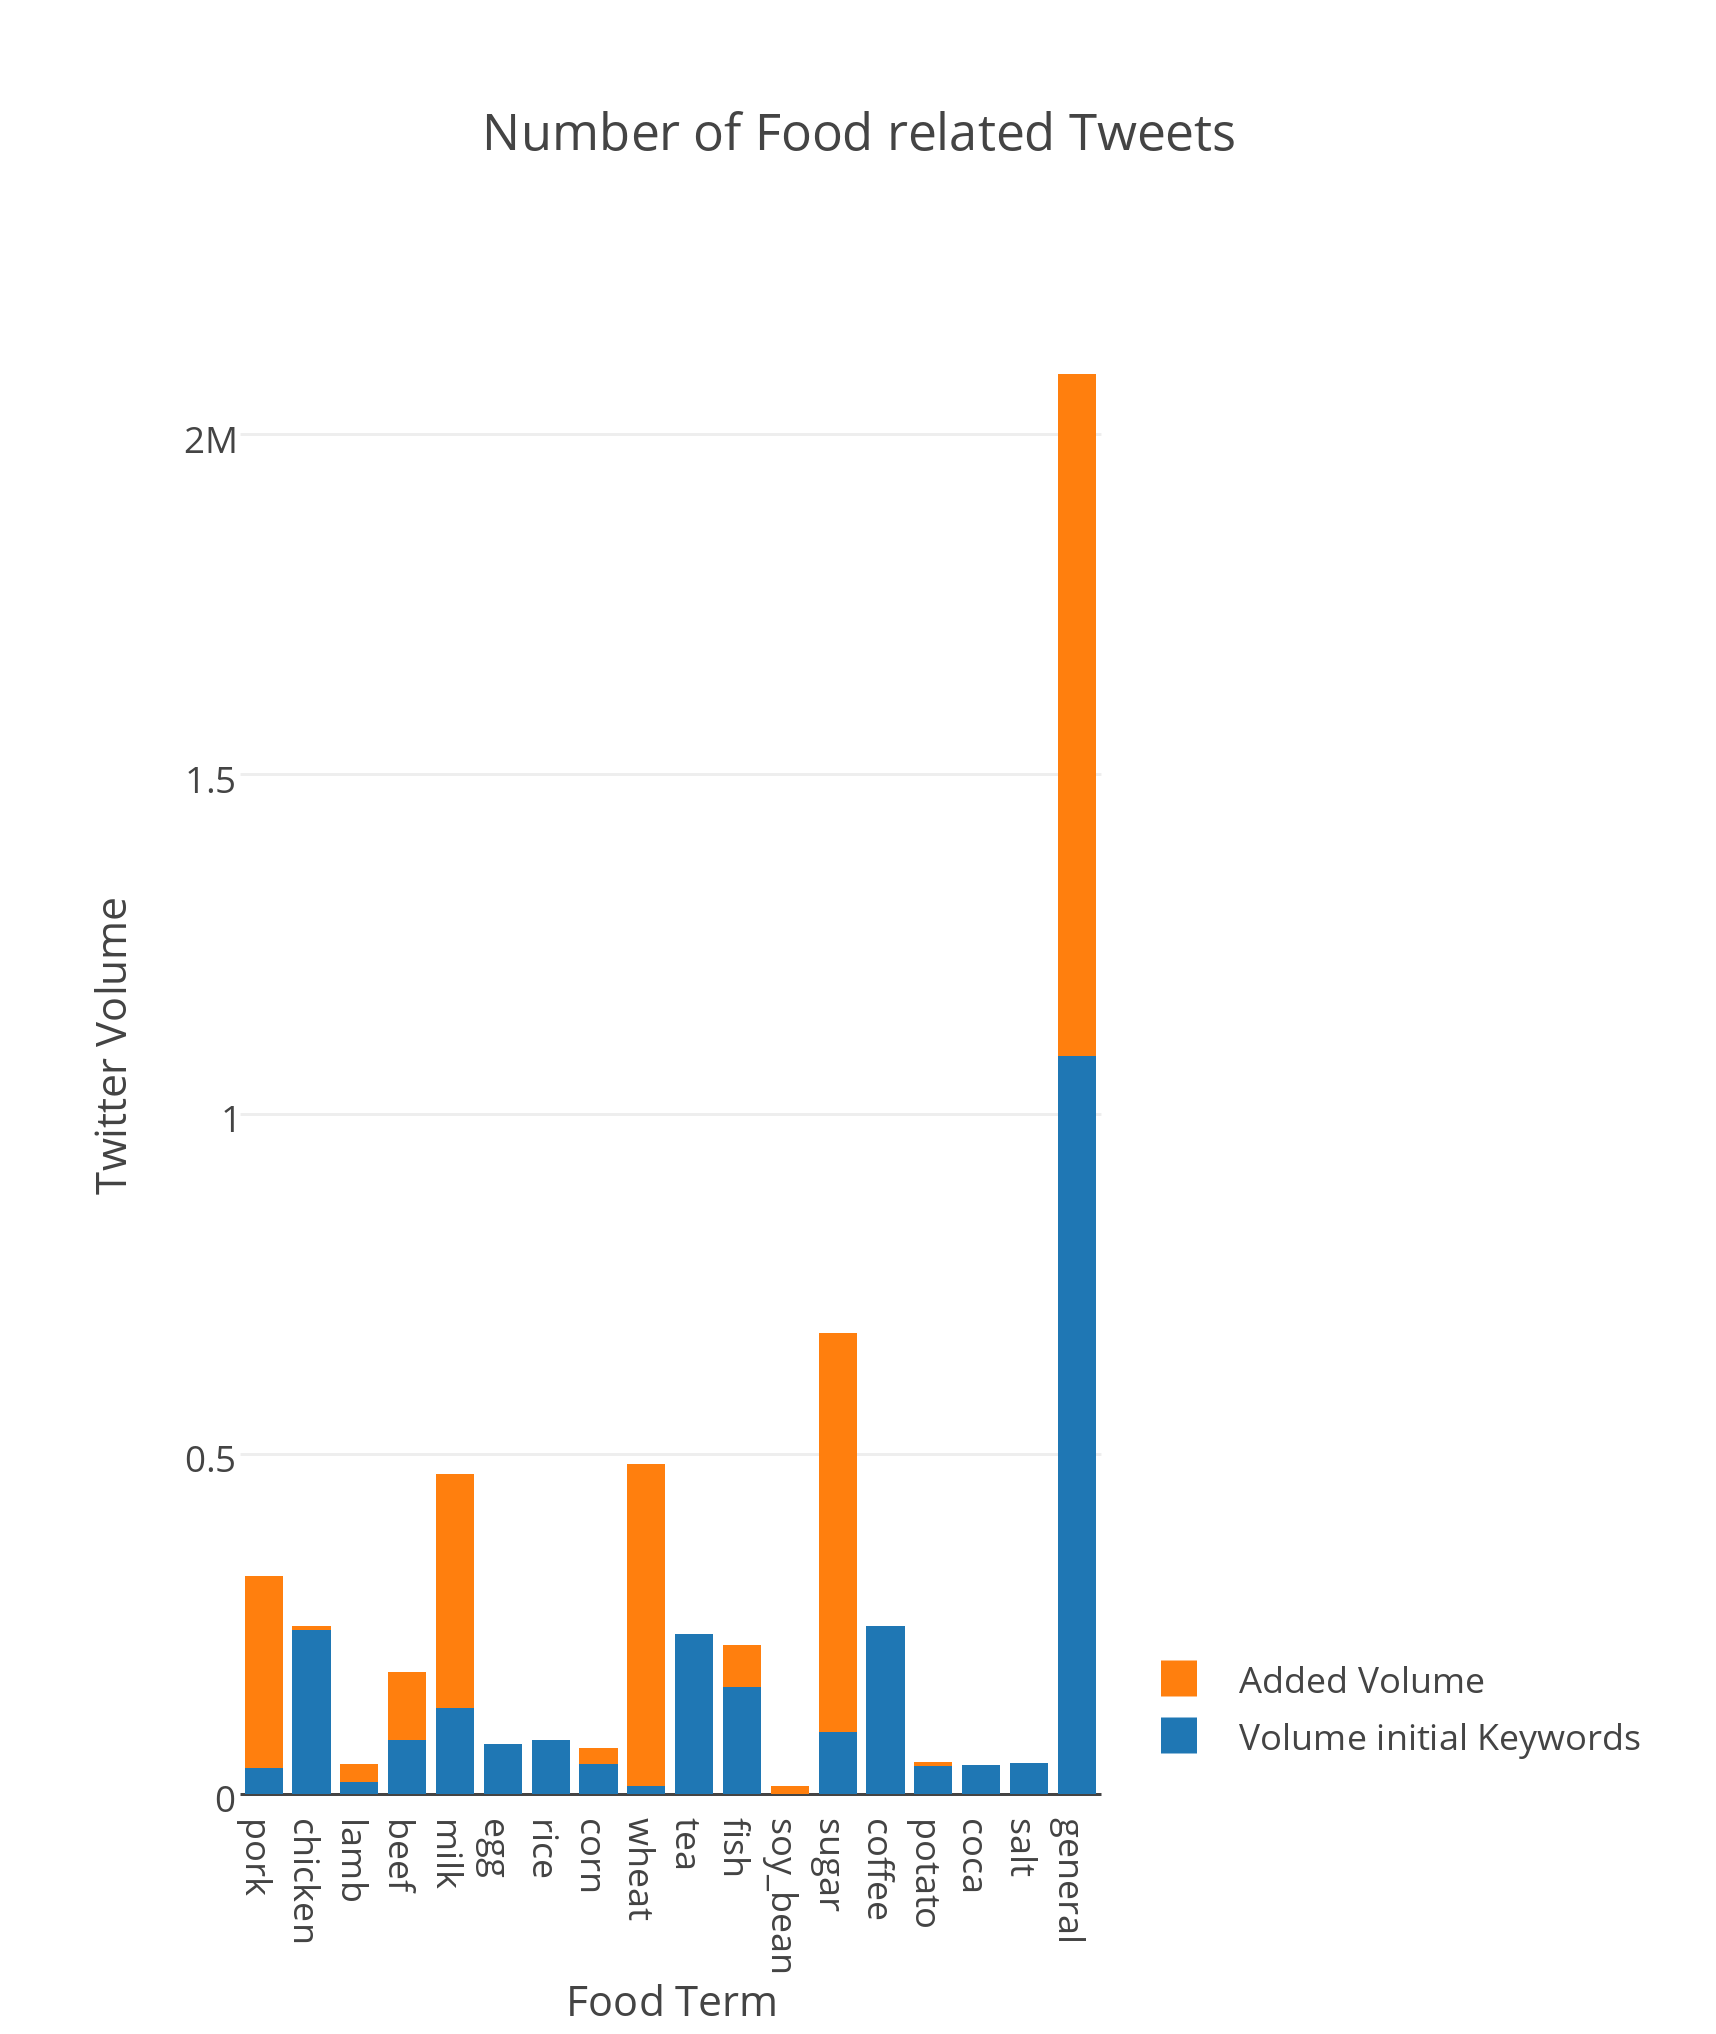
\includegraphics[width=\textwidth]{img/anal/exp_dist}
                \caption{Overall Distribution}
                \label{fig:world}
        \end{subfigure}%
        ~ %add desired spacing between images, e. g. ~, \quad, \qquad, \hfill etc.
          %(or a blank line to force the subfigure onto a new line)
        \begin{subfigure}[b]{0.5\textwidth}
                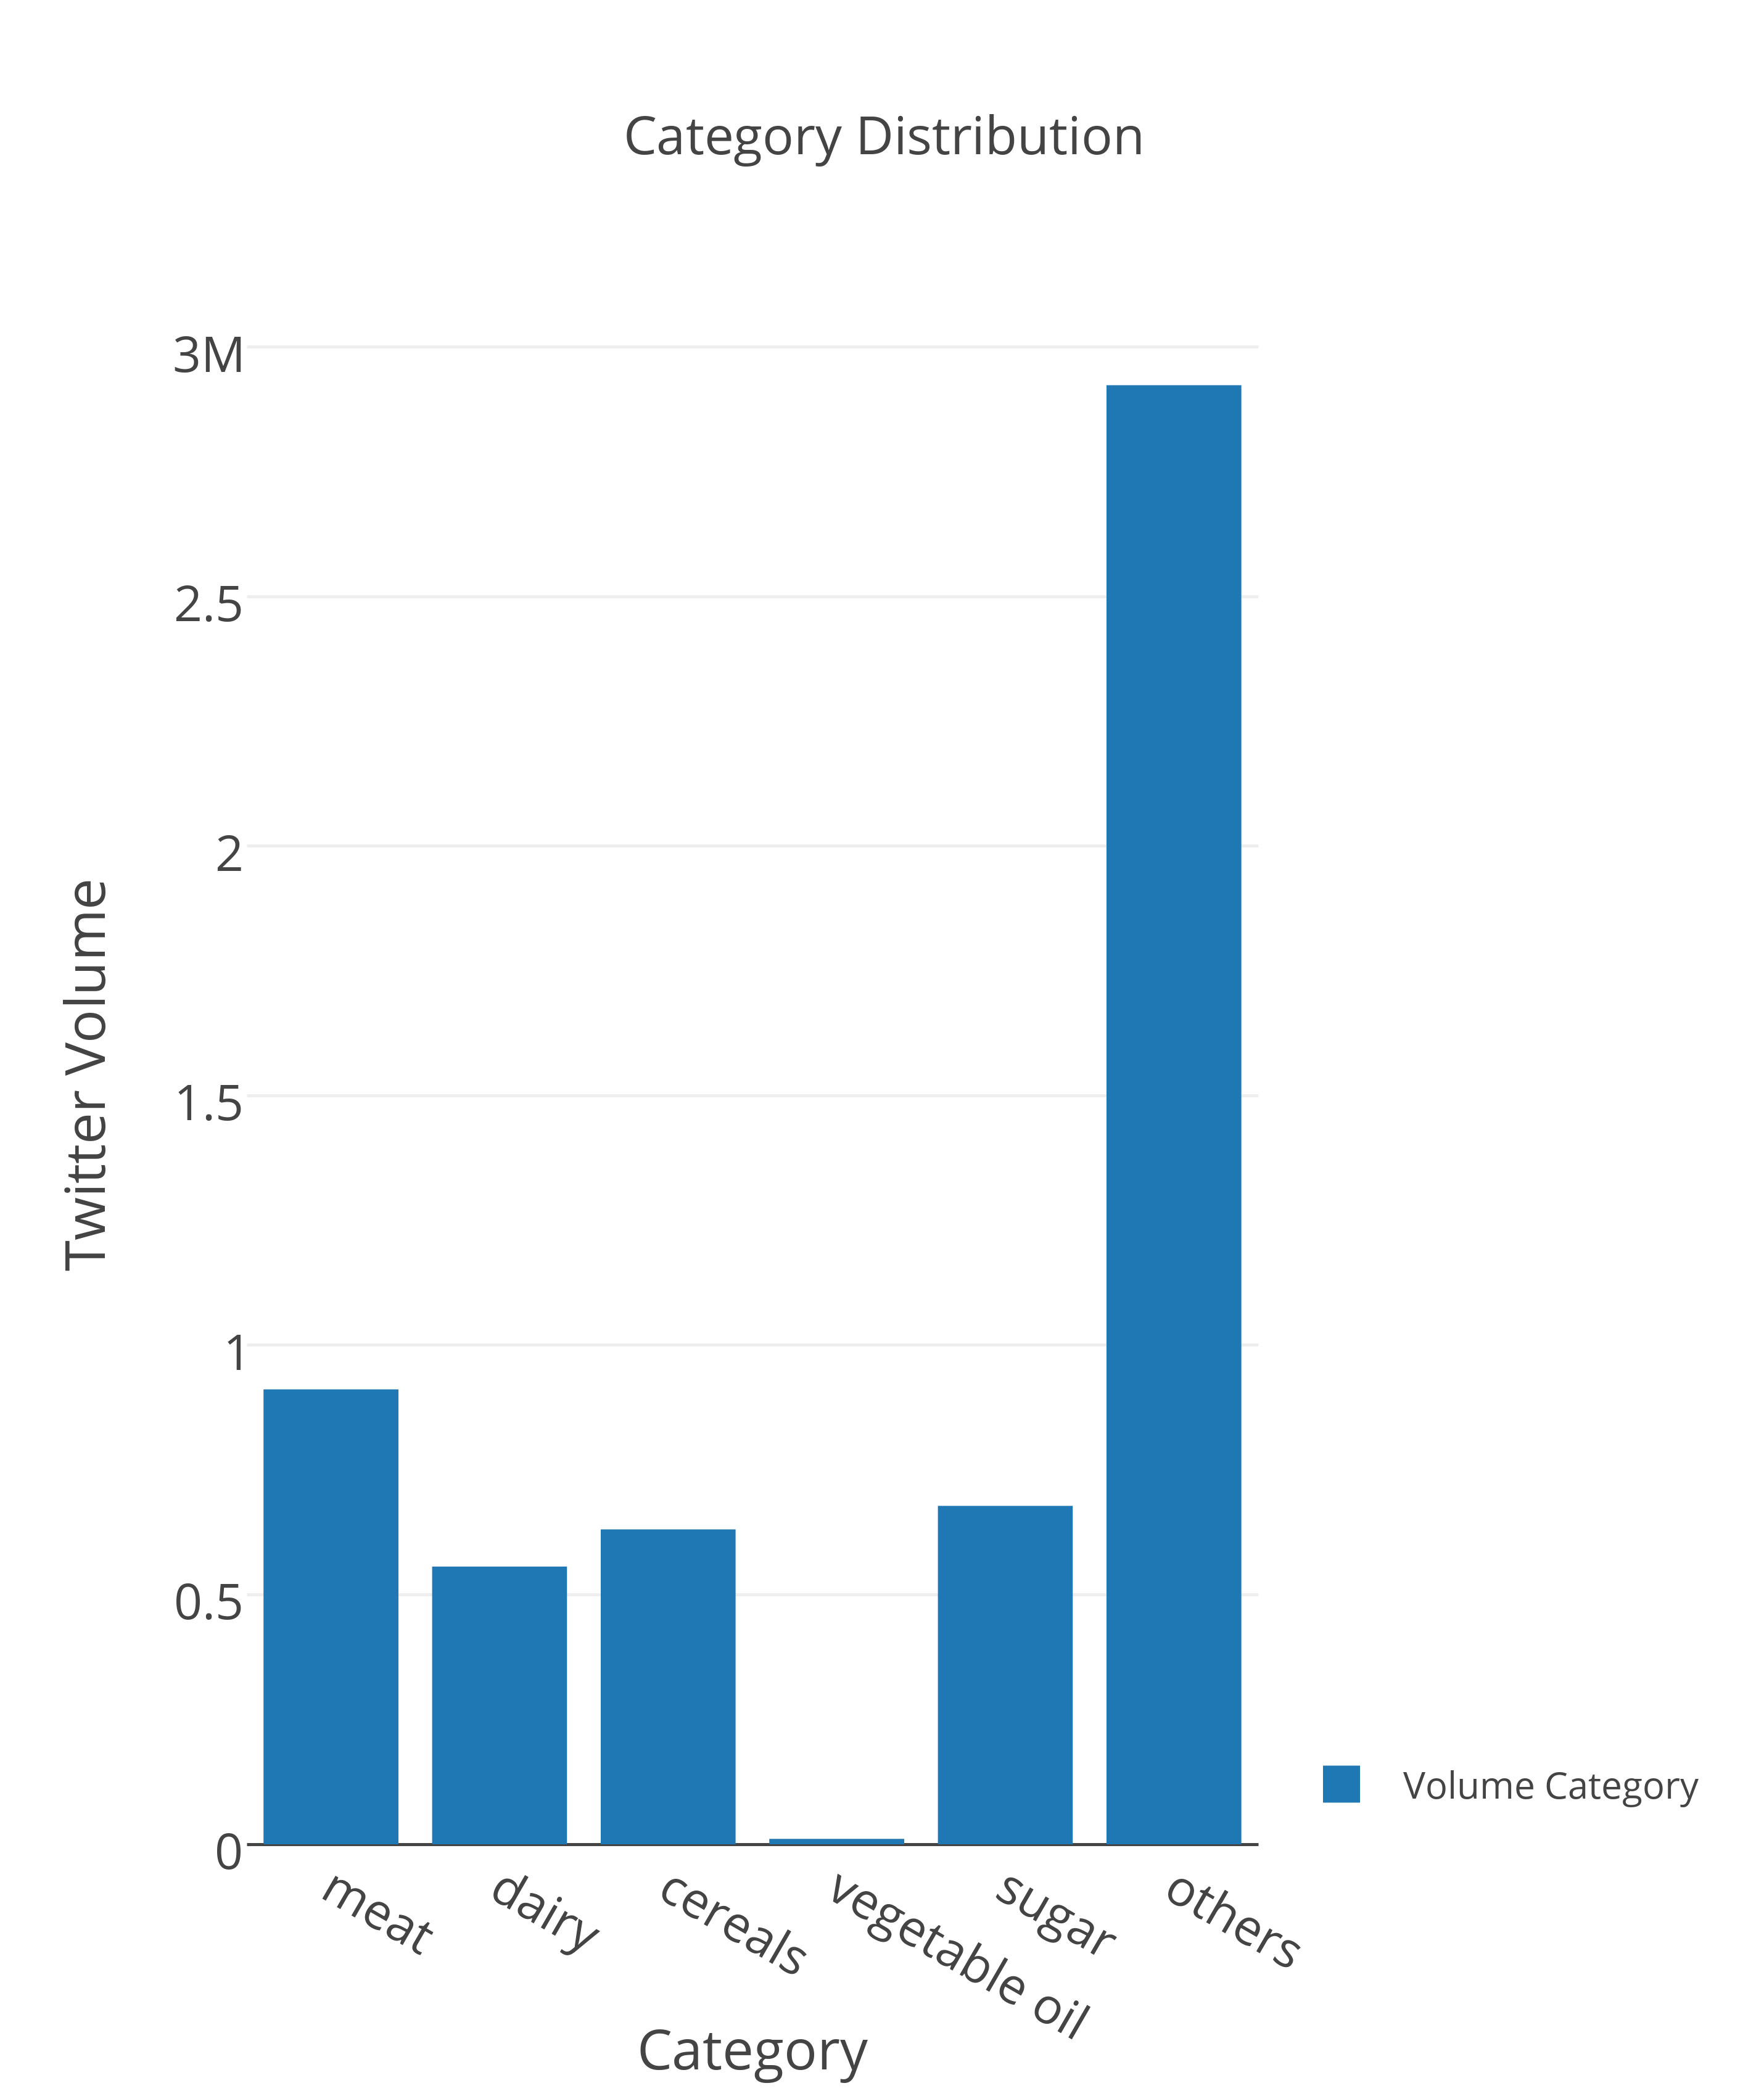
\includegraphics[width=\textwidth]{img/anal/exp_dist_cat}
                \caption{Category Distribution}
                \label{fig:cat}
        \end{subfigure}
        ~ %add desired spacing between images, e. g. ~, \quad, \qquad, \hfill etc.
          %(or a blank line to force the subfigure onto a new line)
      
        \caption{Volume of Tweets per Keyword and per Category}\label{fig:distribution}
\end{figure}


\section{Price Correlation}


We observed the general popularity of food in our initial analysis and that certain food categories have a much stronger presence then others. There is however still a concern on whether the sampled data is useful to detect difference in price fluctuation and lastly can  be used as medium to determine food security. For the purpose of our correlation analysis we used the price quotations of the Food and Argriculture Organisation of the United Nations \footnote{http://www.fao.org/worldfoodsituation/foodpricesindex/en/}. For each food category (e.g. meat, dairy ) we correlated the tweet volumes of the subcategories( e.g. beef, chicken for meat), products (e.g. bacon, salami) and the price quotes for each category. These subcategories mirror the definition of the FAO \cite{fao2008} Since the price quotes of the FAO are based on a monthly average we aggregated the daily tweet volumes over a month and took the average volume per food term. We only included food terms that had an average of greater then 90 tweets per day.  

Between the meat categories there is a strong positive linear relationship in the range of 0.9914 and 0.9980.This means that if chicken increases in volume so does beef and pork. Likewise a p value of 0.0001 suggest that we can reject the idea that the correlation is due to random sampling. A negative relationship exists between the tweet volume and the meat price index ranging from -.469 lamb to -.4855 beef. So a price increase will most likely mean a decrease in tweet volume. Generally speaking we observer a stronger correlation for the meat categories (e.g. beef, chicken) as for meat products (e.g. chorizo, salami). With a p value of ca. 0.003 we again conclude that the correlation is real. 


\begin{figure}[H]
        \centering
         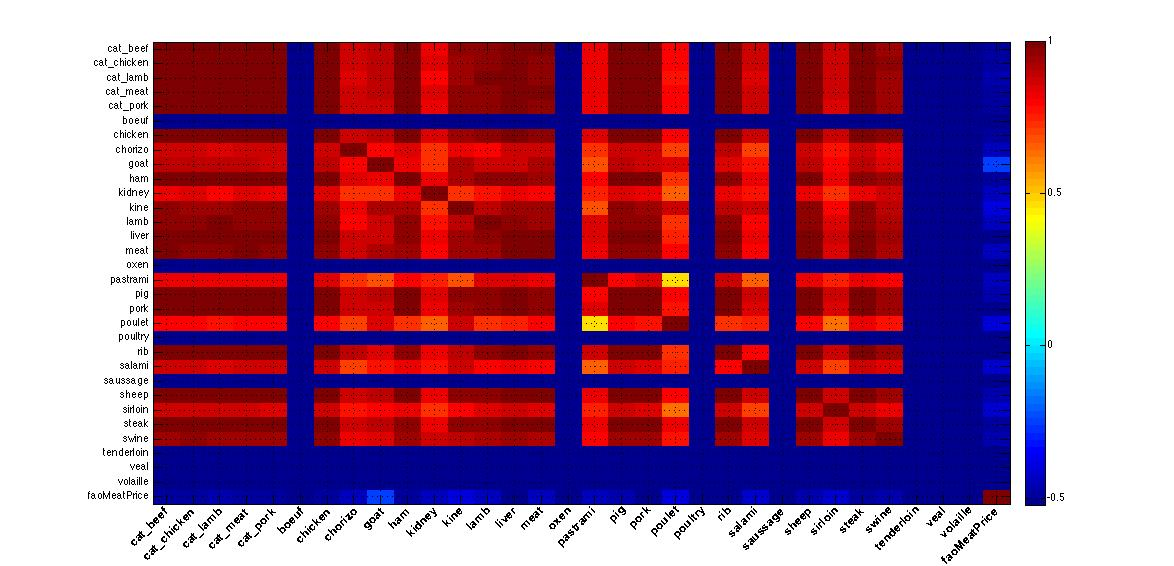
\includegraphics[width=1\textwidth ]{img/anal/meat_heatplot_price}
              
        \caption{Heatplot Meat: Volume of Tweets per Keyword and per Category}
        \label{fig:distribution}
\end{figure}



For cereals similar to meat we likewise see a high correlation in volume of around 0.95 between the different products, the only exception being flower. Interestingly both bread and noodles are made from flower. We can only assume that flour producers hedge the price of wheat and do not pass the price on to bread or noodle producers. Unlike meat products, when we observe an increase in tweet volume for cereals we also observe an increase in the price. The correlation of around 0.65 suggests a stronger relationship between tweet volume and price of cereals then those of meat. 

\begin{figure}[H]
        \centering
         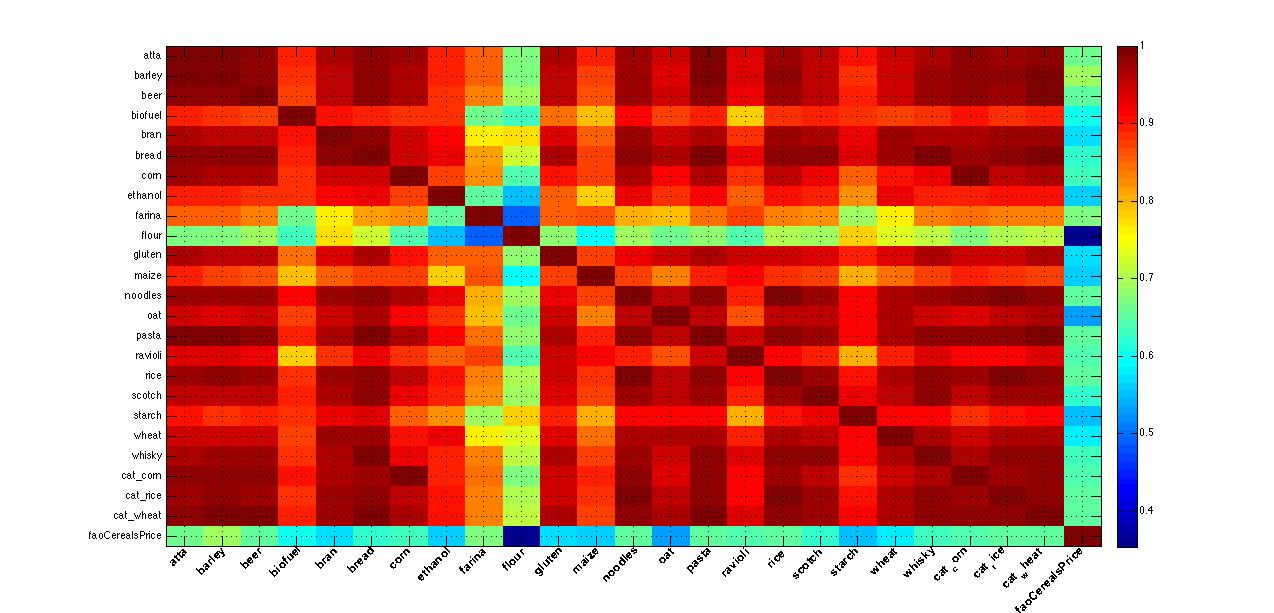
\includegraphics[width=1\textwidth ]{img/anal/cereals_heatplot}
              
        \caption{Heatplot Cereals: Volume of Tweets per Keyword and per Category}
        \label{fig:distribution}
\end{figure}
 
 
 
The heat plot of the dairy products is very similar to the one we observed for meet and has been added to the appendix for reference. An increase in volume of tweets suggests a decrease in price for dairy prices with a correlation of around 0.68. 

\begin{figure}[H]
        \centering
         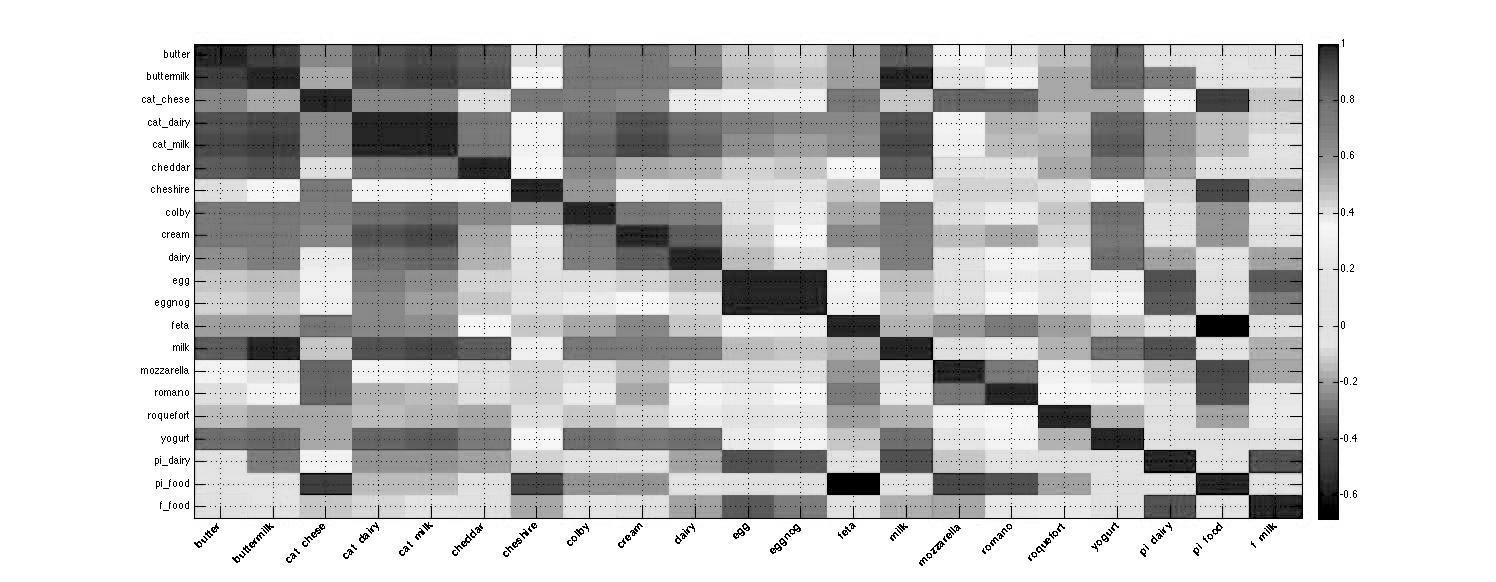
\includegraphics[width=1\textwidth ]{img/anal/dairy_heatplot}
              
        \caption{Heatplot Dairy: Volume of Tweets per Keyword and per Category}
        \label{fig:distribution}
\end{figure}
 
The heat plots of sugar and oil reflect a positive correlation of around 0.37. 

\begin{figure}[H]
        \centering
         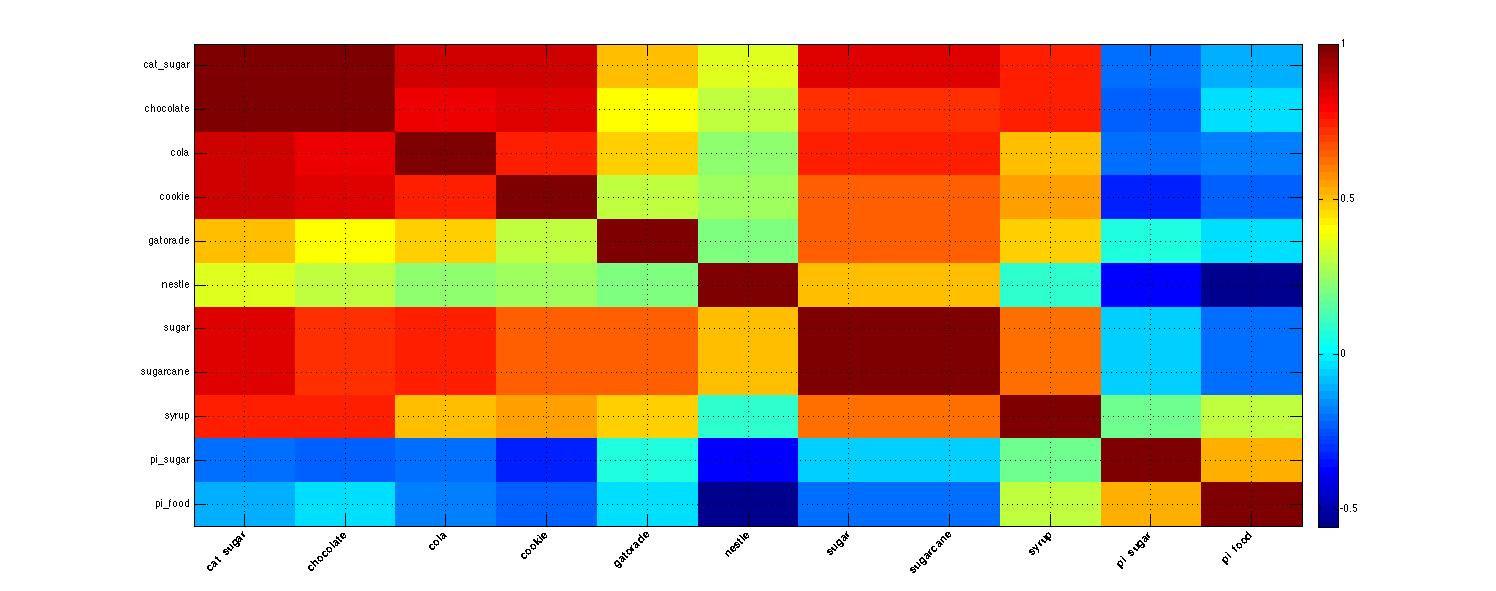
\includegraphics[width=1\textwidth ]{img/anal/sugar_heatplot}
              
        \caption{Heatplot Sugar: Volume of Tweets per Keyword and per Category}
        \label{fig:sugar_heat}
\end{figure}

\begin{figure}[H]
        \centering
         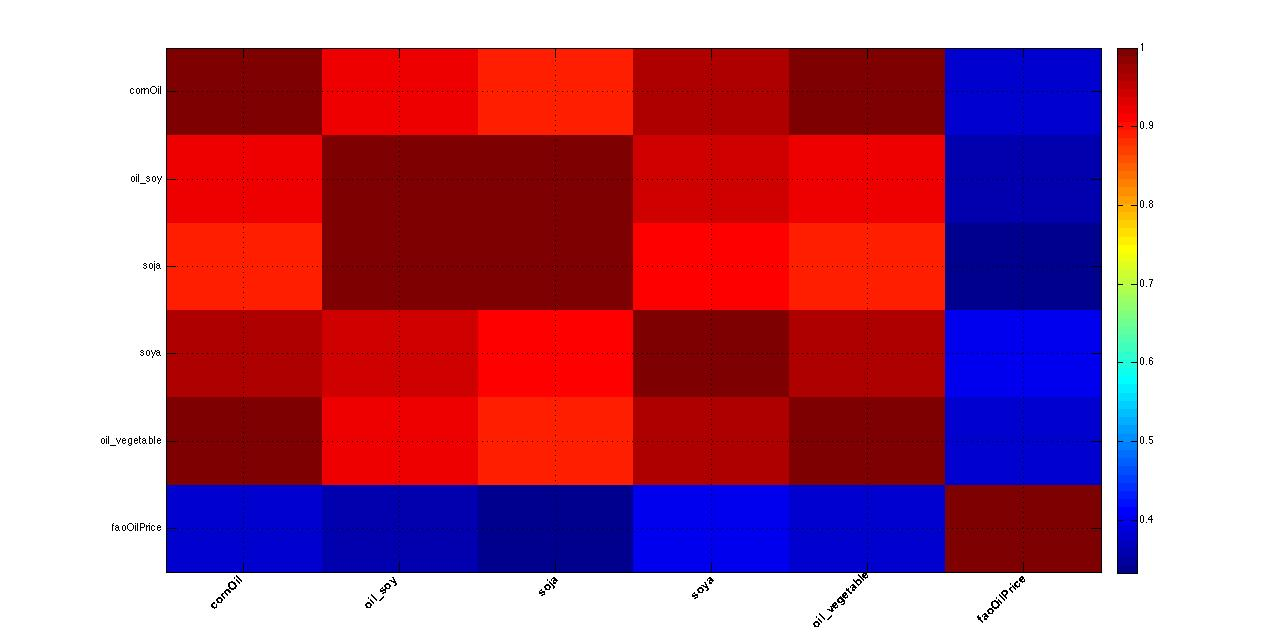
\includegraphics[width=1\textwidth ]{img/anal/oil_heatplot}
              
        \caption{Heatplot Oil: Volume of Tweets per Keyword and per Category}
        \label{fig:oil_heat}
\end{figure}


\subsection{Discussion} 

A smilier correlation analysis has been made in \cite{ungp2013}. They however used more contextual sensitive tweets i.e. instead of just using tweets containing food they performed an n-match on different criteria. The tweet had to contain a food item, the word price and a quantification such as high or low. Overall a pearson correlation of around 0.42 was detected with a significance of 0.04. By looking at the simple raw volume of the tweets we perform significantly better with an average correlation of 0.65 and a p - value of 0.015. Where the correlation for the category prices is significant there is hardly any correlation between the international Food Price Index and the tweet volume of the different categories. This was expected since the International Food Price Index is calculated by a weighted average of the price indices of the five food categories. 
 
 

 
 \begin{center}
 \begin{tabular}{ l | c  | c  }
			
   & \textbf{Category Price Index}  & \textbf{Food Price Index} \\
  \hline
  \\
  Meat & -0.4802 **    & 0.1611  \\
  
  Dairy & -0.7256 ***  & 0.1388\\

  Cereals & 0.6489 *** & 0.1543 \\

  Oil & 0.3804 * &  0.1485  \\

  Sugar & 0.3897 * &0.1881 \\

  General & - & 0.1685 \\
\hline 

\multicolumn{3}{c}{\null}\\

\multicolumn{3}{c}{\textbf{Significance:} p $<$ .0005 ***, p $<$ 0.005 **, p $<$ 0.05 *}\\
\hline  
\end{tabular}
\end{center}


 \section{Anomalie Detection}


Following our correlation analysis we proceed with a detailed investigation of Twitter conversations relevant to food security to uncover events that trigger conversations.  


Traditional market fundamentals such as demand and supply factors were found to be inadequate to explain the recent food crises in 2007 - 2008 and 2010-2011 \cite{abbott2009}. Recent research has been centered around defining causes of soaring food prices such as biofuel demand, trade restrictions or commodity futures markets. In \cite{Tadesse2014} they define a taxonomy for drivers of  international food prices spikes and differentiates among three different causes namely exogenous shocks, conditional causes and internal causes. Examples of exogenous shocks are extreme weather events, oil price shocks, economic and demand/supply growth, and lastly economic shocks. Conditional causes can originate through political conflict or market conditions. Internal causes on the other hand are speculative activities(driven by price expectations) and declines in world food stocks. 

According to \cite{Tadesse2014} , exogenous shocks are expected to generate food price spikes and volatility. The other factors determine the magnitude of the volatility and rely heavily on the political and economic condition of the country. 

Motivated by this research we try to discover spikes in our twitter conversations centered around Food Security and create a link to events that might have 	caused them. Such events can play a significant role in explaining food price volatility. 


\subsection{Methodology} 

We investigate the four food categorie's temporal behaviour on a granularity of one day. This scale was chosen in order to be in accordance with the temporal quotations of the commodity market. Lehmann et al. \cite{Lehmann2012} defines there categories of temporal behaviours. Continuous activity, periodic activity or activity concentrated around an isolated peak. Where continues activities are topics that are of daily  interest such as weather periodic actives reoccur with a fixed pattern such as the release of a new episode of a popular tv show. The later is event driven and usually occurs once during a very short period such as a national holiday. 

In order to detect anomalies in our food topics we applied a similar approach as in \cite{olt15} \cite{Lehmann2012}. A fixed window size of 2m + 1 was defined where $m = 15$ to build a month long time window. Within the window we identified the median and calculated the mean of the twitter volume. From those values we calculated the Median absolute deviation (MAD) as follows: 

\begin{equation} \label{eq:solve}
\overline{ MAD } = median_i (|X_i - median_j(X_j)|)\end{equation}


$X_j$ is the set of data points within the fixed window and $X_i \in X_j$

A peak is declared if $v_i$ deviates more then 1.5 MAD from the mean. For this analysis we only consider rapid increases and ignore anomalies in form of a steep descent. 

The discussion centred around food price showed 147 events, tweet activities for food supply resulted in 160 spikes. 159 anomalies were detected for food needs and lastly 153 for food poverty. 
 

\subsection{Social Attention}

For price and supply we observe a similar temporal pattern. Both show a continuous activity with one extremely prominent event (boost) where the discussion about food supply is followed by a boost in food price. 




\begin{figure}[H]
        \centering
         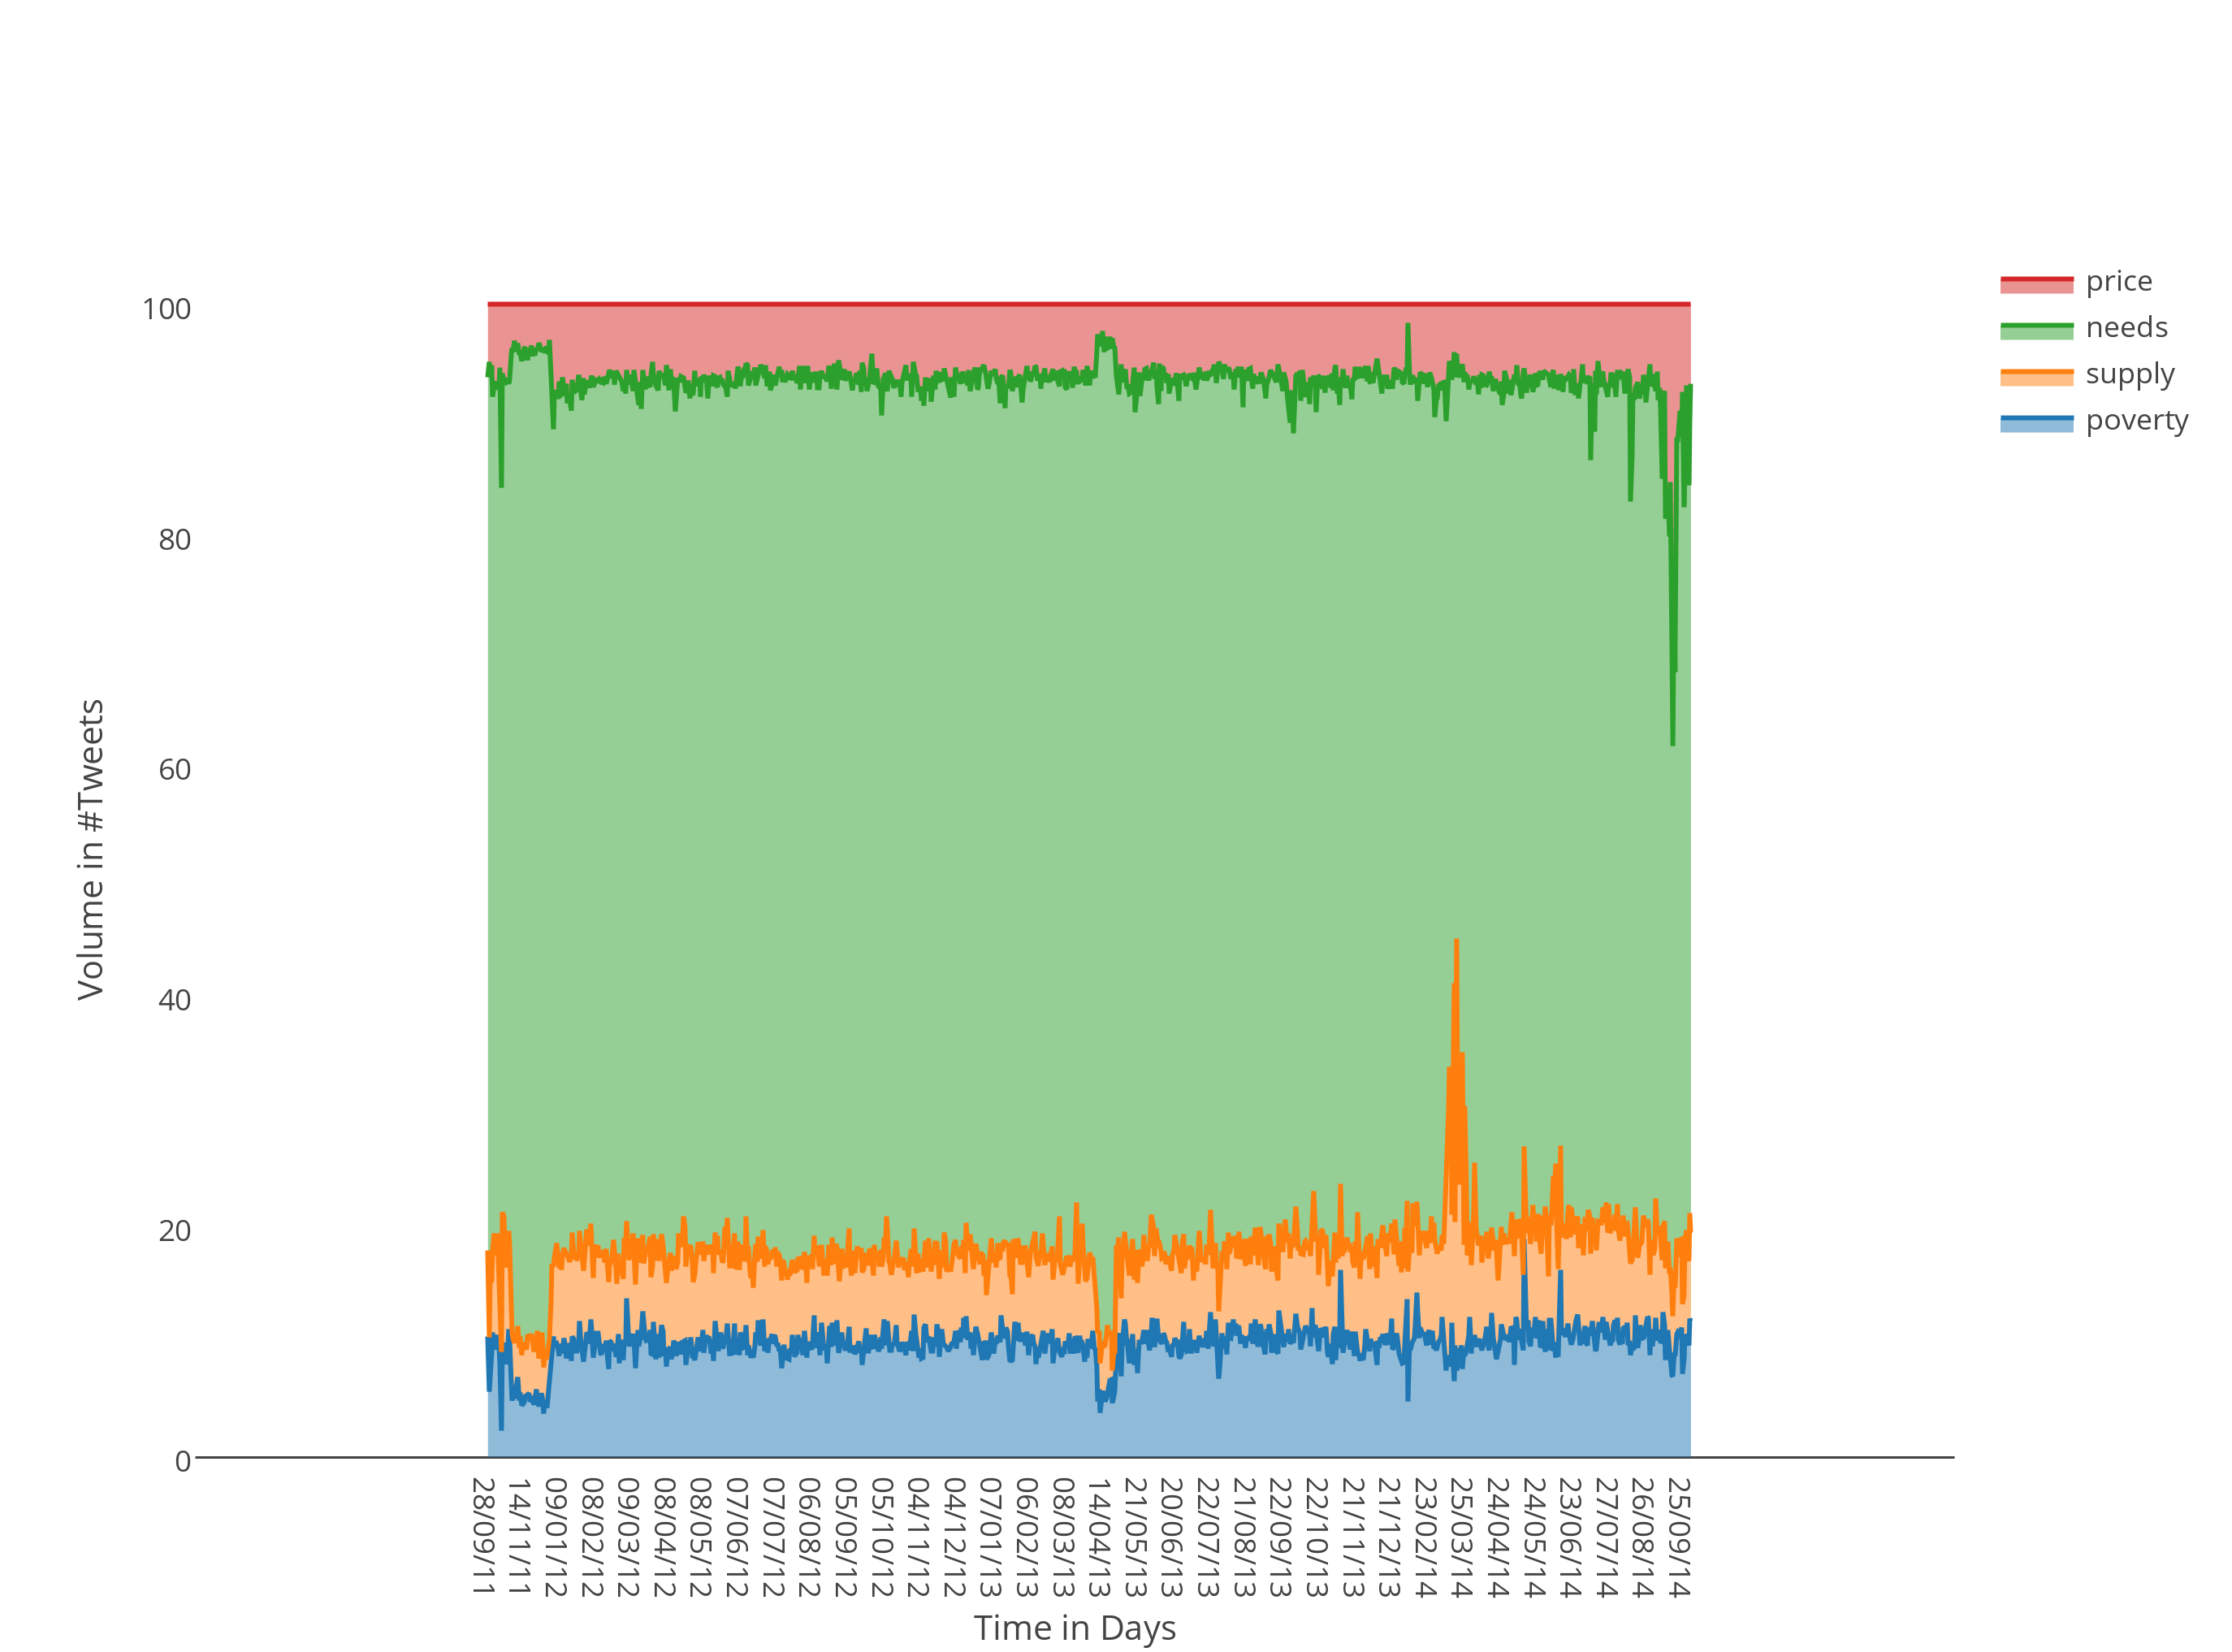
\includegraphics[width=1\textwidth ]{img/anal/topic_dist}
              
        \caption{Topic Distribution - Food Security}
        \label{fig:oil_heat}
\end{figure}

 
\subsection{Event Identification [Not finished]}



The time series data measured in volume per


Burst: 

Investigatng 16092014

Food prices drop to four-year low ? UN agency 

\footnote{http://www.un.org/apps/news/story.asp}


Peak ing at this news article 
16/09/2014: UK Inflation rate down to 1.5 \% \footnote{http://www.bbc.co.uk/news/business-29218855}

investigating 12 and 13.08.14 (exact match)

Oil prices dip to nine-month low: \% \footnote{Oil prices dip to nine-month low}


 
 25/08/12  (exact match)
 
 UPDATE 1-USDA raises beef, pork prices forecasts on drought, disease
 
 
 
 Food supply: 
 
 

exact match(2012/02/23/)
Bill Gates Calls for More Accountability on Food Programs
 \footnote{http://green.blogs.nytimes.com/2012/02/23/bill-gates-calls-for-more-accountability-on-food-programs/}
 
 exact match(05/10/12)
 \footnote{http://www.cnbc.com/id/49301763}
 
 Food Is the New Oil and Land the New Gold: Lester Brown
 
 
21/11/2013
1.7 million in Pa. brace for food stamp reform



%\footnote{http://triblive.com/state/pennsylvania/4741187-74/stamps-stamp-bill#axzz3Zj6QIUuL}
 
 
17/03/2014

Califorinian drought affects food supply	

 \footnote{http://www.latimes.com/food/dailydish/la-dd-california-drought-affecting-food-20140311-story.html}
 


At peak of food supply we have a local high FAO food price






 
